% chktex-file 2% chktex-file 29
% chktex-file 13
\documentclass[12pt]{report}
\usepackage{setspace}
\usepackage[a4paper, total={7in, 10in}]{geometry}
\usepackage[fleqn]{amsmath}
\usepackage{empheq}
\usepackage{amssymb}
\usepackage{amsthm}
\usepackage{gensymb}
\usepackage[fleqn]{cases}
\usepackage{multicol}
\usepackage{color}
\usepackage{stix}
\usepackage{chngcntr}
\usepackage{tikz}
\usepackage{enumitem}
\usepackage{pgfplots}
\usepackage{etoolbox}
\usepackage{tkz-euclide}
\usepackage{graphicx}
\usepackage{enumitem}
\usepackage{multirow}
\usepackage{mathtools}
\usepackage{mdframed}
\usepackage{adjustbox}
\usepackage{xpatch}
\usepackage{nicematrix}
\usepackage{ifthen}

\def\nswe#1#2#3{#1\,$#2^\circ\,#3'$}
\graphicspath{ {./assets/} }
\usetikzlibrary{calc,trees,positioning,arrows,fit,shapes,calc, decorations.markings}
\newcommand{\midarrow}{\tikz \draw[-triangle 90] (0,0) -- +(.1,0);}

\newcommand\typel[2]{
    \mathbin{\mathop{#1\kern0pt}%
        \limits_{\raisebox{3.6ex}{\hbox to0pt{\hss\strut$\uparrow$\hss}}\hbox to0pt{\hss#2\hss}}}
}

\newcommand\typem[2]{
    \mathbin{\mathop{#1\kern0pt}%
        \limits^{\raisebox{3.6ex}{\hbox to0pt{\hss#2\hss}}\hbox to0pt{\hss\strut$\downarrow$\hss}}}
}

\counterwithout{equation}{chapter}

\newcommand{\pgfplotsdrawaxis}{\pgfplots@draw@axis}
\newcommand\perm[2][^n]{\prescript{#1\mkern-2.5mu}{}P_{#2}}
\newcommand\permtwo[2][^n]{{}_{#1}P_{#2}}
\newcommand\comb[2][^n]{{}_{#1}C_{#2}}
\newcommand\combtwo[2][^n]{\prescript{#1\mkern-2.5mu}{}C_{#2}}
\makeatother
\pgfplotsset{only axis on top/.style={axis on top=false, after end axis/.code={
                    \pgfplotsset{axis line style=opaque, ticklabel style=opaque, tick style={thick,opaque},
                        grid=none}\pgfplotsdrawaxis}}}

\newtheorem{theorem}{Theorem}

\makeatletter
\xpatchcmd{\endmdframed}
{\aftergroup\endmdf@trivlist\color@endgroup}
{\endmdf@trivlist\color@endgroup\@doendpe}
{}{}
\makeatother

\mdfdefinestyle{MyFrame}{%
    linecolor=black,
    linewidth=1pt,
    roundcorner=20pt, innertopmargin=20pt,innerbottommargin=20pt, innerrightmargin=12pt,
    innerleftmargin=12pt, skipbelow=20pt, skipabove=20pt
    %backgroundcolor=gray!50!white}
}

\newcommand{\newitem}[1]{%
    \refstepcounter{subenum}%
    \parbox{\dimexpr.5\linewidth-.5\columnsep}{
        \makebox[\labelwidth][r]{(\thesubenum)\hspace*{\labelsep}} #1}\hfill }%%%

\setcounter{chapter}{21}

\setlength{\arrayrulewidth}{1pt}
\setlength{\tabcolsep}{12pt}

\begin{document}

\newcommand{\sol}[1]{

    \noindent \textbf{Sol.}
}
\newcommand{\prooff}[1]{

    \noindent \textbf{Proof.}
}

\newcommand{\sxrightarrow}[2][]{%
    \mathrel{\text{$\xrightarrow[#1]{#2}$}}%
}

\newenvironment{cequation}{
    \makeatletter
    \setbool{@fleqn}{false}
    \makeatother
    \begin{equation*}
        }{\end{equation*}}

\begin{titlepage}
    \raggedleft{}
    \rule{1pt}{\textheight}
    \hspace{0.02\textwidth}
    \parbox[b]{0.75\textwidth}{

    {\fontsize{40}{60}\selectfont\bfseries Mathematics}\\[2\baselineskip]
    {\huge\textit{Senior 3 Part I}}\\[4\baselineskip]
    {\Large\textsc{Melvin Chia}}

    \vspace{0.5\textheight}

    {\noindent Started on 10 April 2023}\\[\baselineskip]
    {\noindent Finished on XX XX 2023}\\[\baselineskip]
    {\noindent Actual time spent: XX days}\\[\baselineskip]}

\end{titlepage}

\chapter*{Introduction}
\addcontentsline{toc}{chapter}{Introduction} \markboth{INTRODUCTION}{}

\doublespacing{}
\section*{Why this book?}

\section*{Disclaimer}
\section*{Acknowledgements}

\singlespacing{}

\doublespacing{}
\tableofcontents
\singlespacing{}
\newpage

\onehalfspacing

\chapter{Exponents and Logarithms}

\section{Exponents}

\subsection*{Definition and Properties of Exponents}

Back in Senior 1, we have learnt the following definitions of exponents:
\begin{flalign*}
    \text{\textbf{Positive exponent}\ \ \ \ \ \ \ }   & a^n = \underbrace{a \times a \times \cdots \times a}_{n \text{ times}}                                 & \\
    \text{\textbf{Zero exponent}\ \ \ \ \ \ \ }       & a^0 = 1                                                                                                & \\
    \text{\textbf{Negative exponent}\ \ \ \ \ \ \ }   & a^{-n} = \dfrac{1}{a^n}\ (a \neq 0, n \in \mathbb{Z}^+)                                                & \\
    \text{\textbf{Fractional exponent}\ \ \ \ \ \ \ } & a^{\frac{m}{n}} = \left(\sqrt[n]{a}\right)^m = \sqrt[n]{a^m}\ (a \geq 0, n > 1, m, n \in \mathbb{Z}^+) &
\end{flalign*}

\noindent The exponent of rational numbers have the following properties:
\begin{enumerate}
    \item $a^m \times a^n = a^{m+n}$
    \item $\dfrac{a^m}{a^n} = a^{m-n}$
    \item $\left(a^m\right)^n = a^{mn}$
    \item $\left(ab\right)^n = a^nb^n$
    \item $\left(\dfrac{a}{b}\right)^n = \dfrac{a^n}{b^n}\ (b \neq 0)$
\end{enumerate}

\newpage

\subsection*{Practice 1}

Without using the calculator, find the value of the following expressions
(Question 1 to 2):
\begin{enumerate}
    \item $2^{-2} + 2{-5} - (-2)^{-3}$
          \sol{}
          \begin{flalign*}
              2^{-2} + 2^{-5} - (-2)^{-3} & = \dfrac{1}{4} + \dfrac{1}{32} - \left(-\dfrac{1}{8}\right) \\
                                          & = \dfrac{8}{32} + \dfrac{1}{32} + \dfrac{4}{32}             \\
                                          & = \dfrac{13}{32}
          \end{flalign*}

    \item $\left(3\dfrac{6}{25}\right)^{-\frac{1}{2}}$
          \sol{}
          \begin{flalign*}
              \left(3\dfrac{6}{25}\right)^{-\frac{1}{2}} & = \left(\dfrac{131}{25}\right)^{-\frac{1}{2}} \\
                                                         & = \dfrac{1}{\sqrt{\dfrac{81}{25}}}            \\
                                                         & = \dfrac{1}{\dfrac{9}{5}}                     \\
                                                         & = \dfrac{5}{9}
          \end{flalign*}

    \item Simplify $a^-4 \div a^{-5} \times (b^{-3})^{-4}$ \sol{}
          \begin{flalign*}
              a^{-4} \div a^{-5} \times (b^{-3})^{-4} & = a^{-4} \times a^5 \times b^{12} \\
                                                      & = a^{-4 + 5} \times b^{12}        \\
                                                      & = ab^{12}
          \end{flalign*}
\end{enumerate}

\newpage

\subsection*{Exponential Functions and Graphs}

Let $a$ is a constant that is bigger than zero and not equal to 1, then the
function being expressed in the form of $y = a^x$ is called an
\emph{exponential function}. The domain of an exponential function is
$\mathbb{R}$.

Consider the following: a cell divides into two cells, and then each of the two
cells divides into two cells again, and so on. If we let $x$ be the number of
divisions, the number of cells after the divisions be $y$, then the functional
relationship between $x$ and $y$ is $y = 2^x$, which is an exponential
function.

In order to look into the graph and its properties of an exponential function
$y = a^x$, we sketch the graph of some exponential functions, the graph of $y =
    2^x$, $y = 10^x$, and $y = \left(\dfrac{1}{2}\right)^x$ are shown in the
diagram below.

\begin{center}
    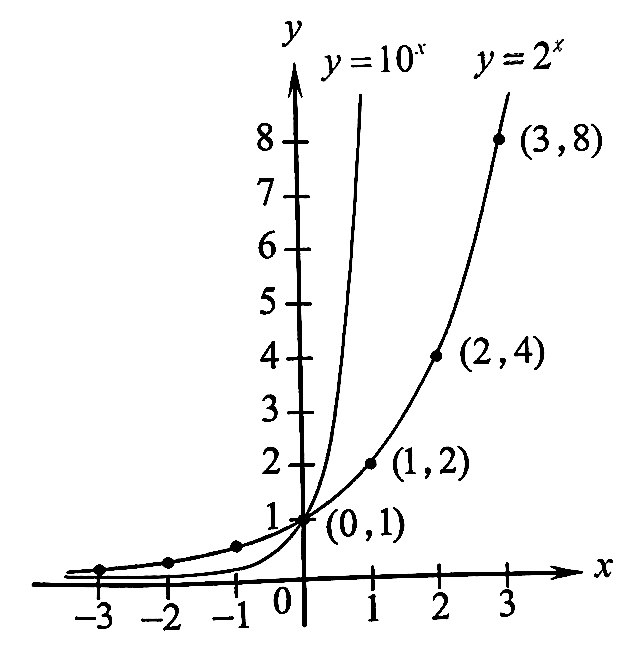
\includegraphics[scale=0.3]{./assets/expo1.jpeg}
    \hspace{1cm}
    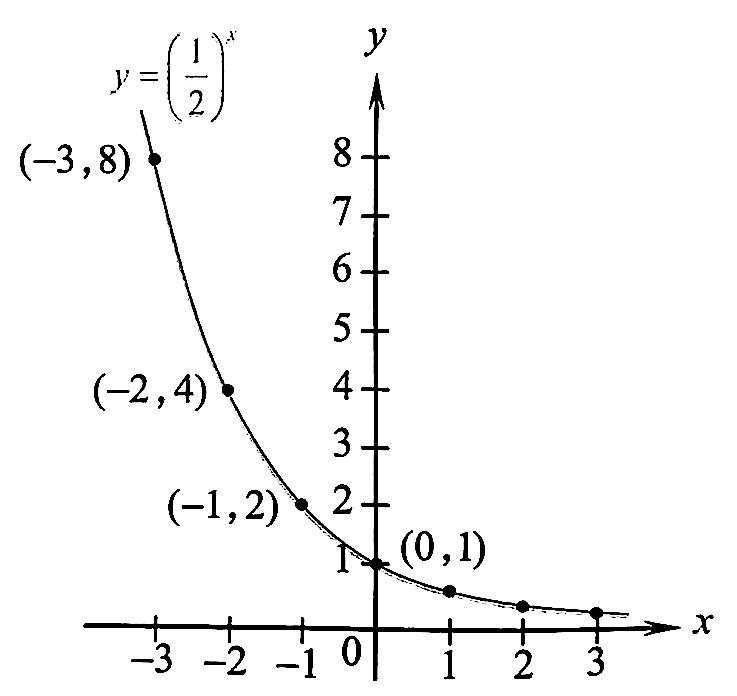
\includegraphics[scale=0.3]{./assets/expo2.jpeg}
\end{center}

From the diagram above, we can see that:
\begin{enumerate}[label=(\arabic*)]
    \item The graph of the function $y = 2^x$, $y = 10^x$, and $y =
              \left(\dfrac{1}{2}\right)^x$ are only at the top of the $x$-axis. Actually,
          when $a > 0$, $a^x > 0$. Therefore, the value of the exponential function $y =
              a^x$ is always positive.

    \item When $x = 0$, $y = 1$. Hence, the graph of exponential functions $y = a^x$
          always passes through the point $(0, 1)$.

    \item For the function $y = 2^x$, when $x > 0$ and $y = 10^x$, when $x < 0$, $y < 1$;
          when $x > 0$, $y > 1$. When the value of $x$ increases, the value of $y$
          increases, that is, the function is an increasing function in the interval
          $(-\infty, +\infty)$.

    \item For the function $y = \left(\dfrac{1}{2}\right)^x$, when $x > 0$, $y > 1$; when
          $x < 0$, $y < 1$. When the value of $x$ increases, the value of $y$ decreases,
          that is, the function is a decreasing function in the interval $(-\infty,
              +\infty)$.
\end{enumerate}

\newpage
When we are discussing about the graph and its properties of an exponential
function $y = a^x$, the following two cases are considered:

\begin{center}
    \begin{NiceTabular}{*{3}{c}}[corners,hvlines]
        & $a > 1$ & $0 < a < 1$ \\
        Graph & 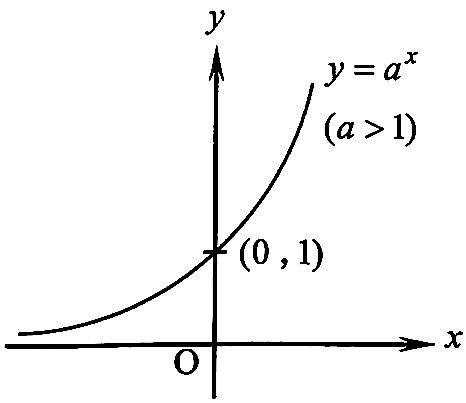
\includegraphics[scale=0.3]{assets/expo3.jpeg} & 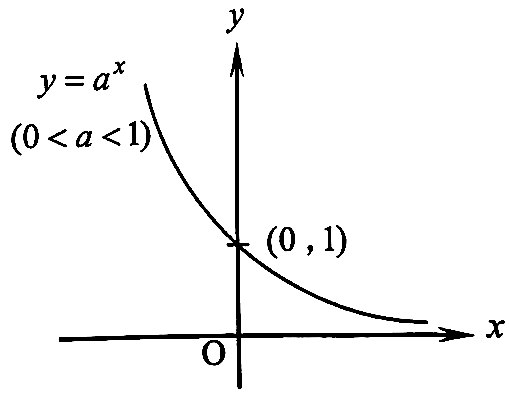
\includegraphics[scale=0.3]{assets/expo4.jpeg} \\
        \Block{4-1}{Properties} & \Block{1-2}{y > 0} \\
        & \Block{1-2}{When $x = 0$, $y = 1$} \\
        & \Block{}{When $x > 0$, $y > 1$;\\When $x < 0$, $0 < y < 1$} & \Block{}{When $x > 0$, $0 < y < 1$;\\When $x < 0$, $y > 1$} \\
        & \Block{}{It is an increasing function in \\the interval $(-\infty, +\infty)$} & \Block{}{It is a decreasing function \\in the interval $(-\infty, +\infty)$} \\
    \end{NiceTabular}
\end{center}

\subsection*{Practice 2}
\begin{enumerate}
    \item Without using the calculator, compare the value of the following expressions:
          \begin{enumerate}
              \begin{multicols}{2}
                  \item $\pi^{2.1}$ and $\pi^{3.5}$
                  \sol{}
                  \begin{flalign*}
                      \because\    & \pi > 1,\ y = \pi^x \text{ is an increasing function}   \\
                                   & \text{in the interval } (-\infty, +\infty)            & \\
                      \because\    & 2.1 < 3.5,                                              \\
                      \therefore\  & \pi^{2.1} < \pi^{3.5}
                  \end{flalign*}

                  \item $0.5^{-2.3}$ and $0.5^{-3.8}$
                  \sol{}
                  \begin{flalign*}
                      \because\    & 0.5 < 1,\ y = 0.5^x \text{ is an increasing function}   \\
                                   & \text{in the interval }  (-\infty, +\infty)           & \\
                      \because\    & -2.3 > -3.8,                                            \\
                      \therefore\  & 0.5^{-2.3} < 0.5^{-3.8}
                  \end{flalign*}
              \end{multicols}
          \end{enumerate}
    \item Given the exponential functions $f(x) = 3^{x^2 - 3x + 5}$ and $g(x) =
              3^{x+10}$. Find the value of $x$ such that $f(x) = g(x)$. \sol{}
          \begin{flalign*}
              f(x) = g(x)                     \\
              3^{x^2 - 3x + 5} = 3^{x+10}     \\
              x^2 - 3x + 5   & = x + 10       \\
              x^2 - 4x - 5   & = 0            \\
              (x - 5)(x + 1) & = 0            \\
              x = 5          & \text{ or } -1
          \end{flalign*}
\end{enumerate}

\subsection*{Exercise 23.1}

Without using the calculator, find the value of the following expressions
(Question 1 to 10):
\begin{enumerate}
    \item $\left(\dfrac{1}{3}\right)^2 + \left(\dfrac{1}{3}\right)^0 - \left(-\dfrac{1}{3}\right)^{-2}$
          \sol{}
          \begin{flalign*}
              \left(\dfrac{1}{3}\right)^2 + \left(\dfrac{1}{3}\right)^0 - \left(-\dfrac{1}{3}\right)^{-2} & = \dfrac{1}{9} + 1 - 9 \\
                                                                                                          & = \dfrac{10}{9} - 9    \\
                                                                                                          & = \dfrac{10 - 81}{9}   \\
                                                                                                          & = -\dfrac{71}{9}
          \end{flalign*}

    \item $\left(\dfrac{3^{-5}\cdot3^{2}}{3^{-3}}\right)^{-2}$
          \sol{}
          \begin{flalign*}
              \left(\dfrac{3^{-5}\cdot3^{2}}{3^{-3}}\right)^{-2} & = \left(\dfrac{3^{-3}}{3^{-3}}\right)^{-2} \\
                                                                 & = 1^{-2}                                   \\
                                                                 & = 1
          \end{flalign*}

    \item $6^{-8} \div 6^{-5} + 3^{-3}$
          \sol{}
          \begin{flalign*}
              6^{-8} \div 6^{-5} + 3^{-3} & = 6^{-8} \times 6^{5} + 3^{-3}    \\
                                          & = 6^{-3} + 3^{-3}                 \\
                                          & = \dfrac{1}{6^3} + \dfrac{1}{3^3} \\
                                          & = \dfrac{1}{216} + \dfrac{1}{27}  \\
                                          & = \dfrac{1 + 8}{216}              \\
                                          & = \dfrac{9}{216}                  \\
                                          & = \dfrac{1}{24}
          \end{flalign*}

          \newpage
    \item $12^{\frac{1}{3}} \times 6^{\frac{1}{3}} \div 27^{\frac{1}{6}} \div 3^{\frac{1}{6}}$
          \sol{}
          \begin{flalign*}
              12^{\frac{1}{3}} \times 6^{\frac{1}{3}} \div 27^{\frac{1}{6}} \div 3^{\frac{1}{6}} & = 72^{\frac{1}{3}} \div 81^{\frac{1}{6}}   \\
                                                                                                 & = 72^{\frac{1}{3}}\div (9^2)^{\frac{1}{6}} \\
                                                                                                 & = 72^{\frac{1}{3}}\div 9^{\frac{1}{3}}     \\
                                                                                                 & = 8^{\frac{1}{3}}                          \\
                                                                                                 & = 2
          \end{flalign*}

    \item $(0.2)^{-2}\times (0.125)^{\frac{2}{3}}$
          \sol{}
          \begin{flalign*}
              (0.2)^{-2}\times (0.125)^{\frac{2}{3}} & = \left(\dfrac{1}{5}\right)^{-2}\times \left(\dfrac{1}{8}\right)^{\frac{2}{3}} \\
                                                     & = 5^2 \times \dfrac{1}{64^{\frac{1}{3}}}                                       \\
                                                     & = 25 \times \dfrac{1}{4}                                                       \\
                                                     & = \dfrac{25}{4}
          \end{flalign*}

    \item $(0.3)^{-\frac{1}{3}}\times(0.0081)^{\frac{1}{3}}+(0.064)^{\frac{1}{3}}$
          \sol{}
          \begin{flalign*}
              (0.3)^{-\frac{1}{3}}\times(0.0081)^{\frac{1}{3}}+(0.064)^{\frac{1}{3}} & = \left(\dfrac{3}{10}\right)^{-\frac{1}{3}} \cdot \left(\dfrac{81}{10000}\right)^{\frac{1}{3}} + \left(\dfrac{64}{1000}\right)^{\frac{1}{3}} \\
                                                                                     & = \left(\dfrac{3}{10}\right)^{-\frac{1}{3}} \cdot \left(\dfrac{3}{10} \cdot \dfrac{27}{1000}\right)^{\frac{1}{3}} + \dfrac{4}{10}            \\
                                                                                     & = \left(\dfrac{3}{10}\right)^{-\frac{1}{3}} \cdot \left(\dfrac{3}{10}\right)^{\frac{1}{3}} \cdot \dfrac{3}{10} + \dfrac{4}{10}               \\
                                                                                     & = \dfrac{3}{10} + \dfrac{4}{10}                                                                                                              \\
                                                                                     & = \dfrac{7}{10}
          \end{flalign*}

          \newpage
    \item $\left(\dfrac{81}{16}\right)^{-\,0.25}\times\left(\dfrac{8}{27}\right)^{-\frac{2}{3}}\times(0.25)^{-2.5}$
          \sol{}
          \begin{flalign*}
              \left(\dfrac{81}{16}\right)^{-\,0.25}\times\left(\dfrac{8}{27}\right)^{-\frac{2}{3}}\times(0.25)^{-2.5} & = \left(\dfrac{16}{81}\right)^{\frac{1}{4}}\times \dfrac{27}{8}^{\frac{2}{3}}\times 4^{\frac{5}{2}} \\
                                                                                                                      & = \dfrac{2}{3}\times \left(\dfrac{3}{2}\right)^2 \times 2^5                                         \\
                                                                                                                      & = \dfrac{2}{3}\times \dfrac{9}{4} \times 32                                                         \\
                                                                                                                      & = 48
          \end{flalign*}

    \item $\left(\dfrac{1}{2}\right)^{-2}+125^{\frac{2}{3}}+343^{\frac{1}{3}}-\left(\dfrac{1}{27}\right)^{-\frac{1}{3}}$
          \sol{}
          \begin{flalign*}
              \left(\dfrac{1}{2}\right)^{-2}+125^{\frac{2}{3}}+343^{\frac{1}{3}}-\left(\dfrac{1}{27}\right)^{-\frac{1}{3}} & = 2^2 + 5^2 + 7 - 3^3 \\
                                                                                                                           & = 4 + 25 + 7 - 3      \\
                                                                                                                           & = 33
          \end{flalign*}
    \item $\left(2{\dfrac{1}{4}}\right)^{-{\frac{3}{2}}}+\left(1{\dfrac{11}{25}}\right)^{-\frac{1}{2}}-\left(2{\dfrac{2}{3}}\right)^{0}$
          \sol{}
          \begin{flalign*}
              \left(2{\dfrac{1}{4}}\right)^{-\frac{3}{2}}+\left(1{\dfrac{11}{25}}\right)^{-1}-\left(2{\dfrac{2}{3}}\right)^{0} & = \left(\dfrac{9}{4}\right)^{-{\frac{3}{2}}}+\left(\dfrac{36}{25}\right)^{-\frac{1}{2}}-1 \\
                                                                                                                               & = \left(\dfrac{2}{3}\right)^3+\dfrac{5}{6}-1                                              \\
                                                                                                                               & = \dfrac{8}{27}+\dfrac{5}{6}-1                                                            \\
                                                                                                                               & = \dfrac{48}{162}+\dfrac{135}{162}-\dfrac{162}{162}                                       \\
                                                                                                                               & = \dfrac{21}{162}                                                                         \\
                                                                                                                               & = \dfrac{7}{54}
          \end{flalign*}

          \newpage
    \item $\dfrac{5\sqrt{4}\sqrt{8}\left({\sqrt[3]{\sqrt[5]{4}}}\right)^{2}}{\sqrt[3]{\sqrt{2}}}$
          \sol{}
          \begin{flalign*}
              \dfrac{\sqrt[5]{4}\sqrt{8}\left({\sqrt[3]{\sqrt[5]{4}}}\right)^{2}}{\sqrt[3]{\sqrt{2}}} & = \dfrac{\left(\sqrt[5]{2}\right)^2\left(\sqrt{2}\right)^3\left(\sqrt[15]{2}\right)^4}{\sqrt[6]{2}} \\
                                                                                                      & = \dfrac{2^{\frac{2}{5}}\cdot 2^{\frac{3}{2}}\cdot 2^{\frac{4}{15}}}{2^{\frac{1}{6}}}               \\
                                                                                                      & = 2^{\frac{2}{5}+\frac{3}{2}+\frac{4}{15}-\frac{1}{6}}                                              \\
                                                                                                      & = 2^{\frac{12+45+8-5}{30}}                                                                          \\
                                                                                                      & = 2^{\frac{60}{30}}                                                                                 \\
                                                                                                      & = 2^2                                                                                               \\
                                                                                                      & = 4
          \end{flalign*}
\end{enumerate}

\noindent Simplify the following expressions (Question 11 to 24):
\begin{enumerate}
    \setcounter{enumi}{10}
    \item $a^{\frac{1}{2}}\cdot a^{\frac{1}{4}}\cdot a^{-{\frac{1}{8}}}\cdot a^{\frac{1}{6}}$
          \sol{}
          \begin{flalign*}
              a^{\frac{1}{2}}\cdot a^{\frac{1}{4}}\cdot a^{-{\frac{1}{8}}}\cdot a^{\frac{1}{6}} & = a^{\frac{1}{2}+\frac{1}{4}-\frac{1}{8}+\frac{3}{8}} \\
                                                                                                & = a^{\frac{12+6-3+9}{24}}                             \\
                                                                                                & = a^{\frac{24}{24}}                                   \\
                                                                                                & = a
          \end{flalign*}

    \item $\left(9a^{2}b^{-2}c^{-4}\right)^{-1}$
          \sol{}
          \begin{flalign*}
              \left(9a^{2}b^{-2}c^{-4}\right)^{-1} & = \dfrac{1}{9a^{2}b^{-2}c^{-4}} \\
                                                   & = \dfrac{b^{2}c^{4}}{9a^{2}}
          \end{flalign*}

          \newpage
    \item $\left(x^{4}y^{-5}\right)\left(x^{-2}y^{2}\right)^{2}$
          \sol{}
          \begin{flalign*}
              \left(x^{4}y^{-5}\right)\left(x^{-2}y^{2}\right)^{2} & = x^{4}y^{-5}x^{-4}y^{4} \\
                                                                   & = x^{4-4}y^{-5+4}        \\
                                                                   & = y^{-1}                 \\
                                                                   & = \dfrac{1}{y}
          \end{flalign*}

    \item $3a^{-2}b^{-3}\div\left(-3^{-1}a^{2}b^{-3}\right)$
          \sol{}
          \begin{flalign*}
              3a^{-2}b^{-3}\div\left(-3^{-1}a^{2}b^{-3}\right) & = \dfrac{3a^{-2}b^{-3}}{-\dfrac{1}{3}a^{2}b^{-3}} \\
                                                               & = -\dfrac{9}{a^{4}}
          \end{flalign*}

    \item $\sqrt[3]{\dfrac{a^{2}b^{-1}}{a^{\frac{1}{2}}b^{5}}}$
          \sol{}
          \begin{flalign*}
              \sqrt[3]{\dfrac{a^{2}b^{-1}}{a^{\frac{1}{2}}b^{5}}} & = \sqrt[3]{a^2b^{-1}a^{-\frac{1}{2}}b^{-5}}      \\
                                                                  & = \left(a^\frac{3}{2}b^{-6}\right)^{\frac{1}{3}} \\
                                                                  & = a^\frac{1}{2}b^{-2}                            \\
                                                                  & = \dfrac{\sqrt{a}}{b^2}
          \end{flalign*}

    \item $5a^{-2}b^{-3}\div\left(5^{-1}a^{2}b^{-3}\right)\times 5^{-2}a b^{4}c$
          \sol{}
          \begin{flalign*}
              5a^{-2}b^{-3}\div\left(5^{-1}a^{2}b^{-3}\right)\times 5^{-2}a b^{4}c & = 5^{1 - (-1) - 2}a^{-2 - 2 + 1}b^{-3 - (-3) + 4}c \\
                                                                                   & = a^{-3}b^{4}c                                     \\
                                                                                   & = \dfrac{b^4c}{a^3}
          \end{flalign*}

          \newpage
    \item $\dfrac{a^{-2}-b^{-2}}{a^{-2}+b^{-2}}$
          \sol{}
          \begin{flalign*}
              \dfrac{a^{-2}-b^{-2}}{a^{-2}+b^{-2}} & = \dfrac{a^{-2}-b^{-2}}{a^{-2}+b^{-2}}\cdot\dfrac{a^2b^2}{a^2b^2} \\
                                                   & = \dfrac{a^{-2}a^2b^2-b^{-2}a^2b^2}{a^{-2}a^2b^2+b^{-2}a^2b^2}    \\
                                                   & = \dfrac{b^2-a^2}{b^2+a^2}
          \end{flalign*}

    \item $\left(a^{-1}+b^{-1}\right)\left(a+b\right)^{-1}$
          \sol{}
          \begin{flalign*}
              \left(a^{-1}+b^{-1}\right)\left(a+b\right)^{-1} & = \dfrac{a^{-1}+b^{-1}}{a+b}                    \\
                                                              & = \dfrac{a^{-1}+b^{-1}}{a+b}\cdot\dfrac{ab}{ab} \\
                                                              & = \dfrac{b+a}{ab\left(a+b\right)}               \\
                                                              & = \dfrac{1}{ab}
          \end{flalign*}

    \item $\left(x+x^{-1}\right)\left(x-x^{-1}\right)$
          \sol{}
          \begin{flalign*}
              \left(x+x^{-1}\right)\left(x-x^{-1}\right) & = x^2 - 1 + 1 - x^{-2} \\
                                                         & = x^2 - x^{-2}         \\
                                                         & = x^2 - \dfrac{1}{x^2} \\
                                                         & = \dfrac{x^4 - 1}{x^2}
          \end{flalign*}

    \item $\left(-2x^{\frac{1}{4}}y^{-\frac{1}{3}}\right)\left(3x^{-\frac{1}{2}}y^{\frac{2}{3}}\right)\left(-4x^{\frac{1}{4}}y^{\frac{2}{3}}\right)$
          \sol{}
          \begin{flalign*}
              \left(-2x^{\frac{1}{4}}y^{-\frac{1}{3}}\right)\left(3x^{-\frac{1}{2}}y^{\frac{2}{3}}\right)\left(-4x^{\frac{1}{4}}y^{\frac{2}{3}}\right) & = -2\times3\times(-4)x^{\frac{1}{4}-\frac{1}{2}+\frac{1}{4}}y^{-\frac{1}{3}+\frac{2}{3}+\frac{2}{3}} \\
                                                                                                                                                       & = 24x^0y^1                                                                                           \\
                                                                                                                                                       & = 24y
          \end{flalign*}

          \newpage
    \item $2x^{-{\frac{1}{3}}}\left({\dfrac{1}{2}}x^{{\frac{1}{3}}}-2x^{-{\frac{2}{3}}}\right)$
          \sol{}
          \begin{flalign*}
              2x^{-{\frac{1}{3}}}\left({\dfrac{1}{2}}x^{{\frac{1}{3}}}-2x^{-{\frac{2}{3}}}\right) & = x^{-{\frac{1}{3}}}x^{{\frac{1}{3}}}-x^{-{\frac{1}{3}}}4x^{-{\frac{2}{3}}} \\
                                                                                                  & = x^0 - 4x^{-1}                                                             \\
                                                                                                  & = 1 - \dfrac{4}{x}                                                          \\
                                                                                                  & = \dfrac{x-4}{x}
          \end{flalign*}

    \item $\left(\sqrt[3]{x^{3}}\cdot\sqrt{y}\right)^{2}\cdot\left(\sqrt{y}\cdot\sqrt{x^{3}}\right)^{3}$
          \sol{}
          \begin{flalign*}
              \left(\sqrt[3]{x^{3}}\cdot\sqrt{y}\right)^{2}\cdot\left(\sqrt{y}\cdot\sqrt{x^{3}}\right)^{3} & = \left(xy^{\frac{1}{2}}\right)^2\cdot\left(y^{\frac{1}{2}}x^{\frac{3}{2}}\right)^3 \\
                                                                                                           & = x^2y\cdot y^{\frac{3}{2}}x^{\frac{9}{2}}                                          \\
                                                                                                           & = x^{\frac{13}{2}}y^{\frac{5}{2}}                                                   \\
                                                                                                           & = x^6y^2\sqrt{xy}
          \end{flalign*}

    \item $\dfrac{3\times2^{n}-4\times2^{n-2}}{2^{n}-2^{n-1}}$
          \sol{}
          \begin{flalign*}
              \dfrac{3\times2^{n}-4\times2^{n-2}}{2^{n}-2^{n-1}} & = \dfrac{3 \times 2^n - 4 \times 2^n \times 2^{-2}}{2^n - 2^n \times 2^-1} \\
                                                                 & = \dfrac{3 \times 2^n - 2^n}{2^n\left(1-  \dfrac{1}{2}\right)}             \\
                                                                 & = \dfrac{2\times 2^n}{\dfrac{1}{2}\times 2^n}                              \\
                                                                 & = 4
          \end{flalign*}

    \item $\left(3^{n+6}-5\times3^{n+1}\right)\div\left(7\times3^{n+2}\right)$
          \sol{}
          \begin{flalign*}
              \left(3^{n+6}-5\times3^{n+1}\right)\div\left(7\times3^{n+2}\right) & = \dfrac{3^n\times3^6-5\times3^n\times3}{7\times3^{n}\times 9} \\
                                                                                 & = \dfrac{3^n\left(3^6-15\right)}{63\times3^n}                  \\
                                                                                 & = \dfrac{3^6-15}{63}                                           \\
                                                                                 & = \dfrac{34}{3}
          \end{flalign*}
    \item Sketch the graph of the following functions on the same diagram:
          \begin{enumerate}[label=(\alph*)]
              \item $y = 3^x$
              \item $y = \left(\dfrac{1}{3}\right)^x$
          \end{enumerate}
          \sol{}
          \begin{center}
              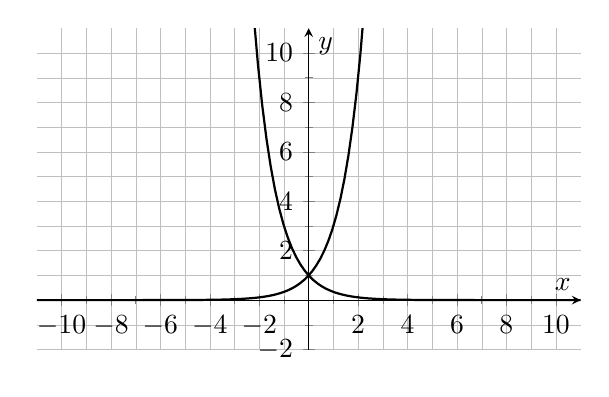
\begin{tikzpicture}
                  \begin{axis}[
                          unit vector ratio*=1 1 1,
                          axis lines = middle,
                          xlabel = $x$,
                          ylabel = $y$,
                          ymin = -2,
                          ymax = 11,
                          xmin = -11,
                          xmax = 11,
                          xtick = {-10, -8,...,10},
                          ytick = {-2,0,...,10},
                          minor tick num = 1,
                          grid = both,
                          grid style = {line width=.1pt, draw=gray!50},
                          major grid style = {line width=.2pt,draw=gray!50},
                          width = 0.7\textwidth,
                      ]
                      \addplot [
                          domain=-11:5,
                          samples=100,
                          thick,
                      ]
                      {3^x};
                      \addplot [
                          domain=-6:11,
                          samples=100,
                          thick,
                      ]
                      {(1/3)^x};
                  \end{axis}
              \end{tikzpicture}
          \end{center}

    \item Without using the calculator, compare the value of the following expressions:
          \begin{enumerate}
              \begin{multicols}{2}
                  \item $2.5^{7.1}$ and $2.5^{8.5}$
                  \sol{}
                  \begin{flalign*}
                      \because   & \ 2.5 > 1,\ y = 2.5^x\ \text{is an increasing}                & \\
                                 & \text{function in the interval } \left(-\infty, \infty\right)   \\
                      \because   & \ 7.1 < 8.5,                                                    \\
                      \therefore & \ 2.5^{7.1} < 2.5^{8.5}
                  \end{flalign*}

                  \item $0.35^{6.5}$ and $0.35^{5.6}$
                  \sol{}
                  \begin{flalign*}
                      \because   & \ 0.35 < 1,\ y = 0.35^x\ \text{is a decreasing}               & \\
                                 & \text{function in the interval } \left(-\infty, \infty\right)   \\
                      \because   & \ 6.5 > 5.6,                                                    \\
                      \therefore & \ 0.35^{6.5} < 0.35^{5.6}
                  \end{flalign*}
              \end{multicols}

              \begin{multicols}{2}
                  \item $1.03^{-2.1}$ and $1.03^{-3.2}$
                  \sol{}
                  \begin{flalign*}
                      \because   & \ 1.03 > 1,\ y = 1.03^x\ \text{is an increasing}              & \\
                                 & \text{function in the interval } \left(-\infty, \infty\right)   \\
                      \because   & \ -2.1 > -3.2,                                                  \\
                      \therefore & \ 1.03^{-2.1} < 1.03^{-3.2}
                  \end{flalign*}

                  \item $\left(\sqrt{2}\right)^\pi$ and $\left(\sqrt{2}\right)^{\pi - 3.5}$
                  \sol{}
                  \begin{flalign*}
                      \because   & \ \sqrt{2} > 1,\ y = \left(\sqrt{2}\right)^x\ \text{is an increasing} & \\
                                 & \text{function in the interval } \left(-\infty, \infty\right)           \\
                      \because   & \ \pi > \pi - 3.5,                                                      \\
                      \therefore & \ \left(\sqrt{2}\right)^\pi > \left(\sqrt{2}\right)^{\pi - 3.5}
                  \end{flalign*}
              \end{multicols}

              \newpage
              \begin{multicols}{2}
                  \item $0.01^{-\frac{1}{3}}$ and $0.01^{-\frac{1}{2}}$
                  \sol{}
                  \begin{flalign*}
                      \because   & \ 0.01 < 1,\ y = 0.01^x\ \text{is a decreasing}               & \\
                                 & \text{function in the interval } \left(-\infty, \infty\right)   \\
                      \because   & \ -\dfrac{1}{3} > -\dfrac{1}{2},                                \\
                      \therefore & \ 0.01^{-\frac{1}{3}} < 0.01^{-\frac{1}{2}}
                  \end{flalign*}

                  \item $2.7^{\sqrt{20}}$ and $2.7^{\sqrt[3]{35}}$
                  \sol{}
                  \begin{flalign*}
                      \because   & \ 2.7 > 1,\ y = 2.7^x\ \text{is an increasing}                & \\
                                 & \text{function in the interval } \left(-\infty, \infty\right)   \\
                      \because   & \ \sqrt{20} > \sqrt[3]{35},                                     \\
                      \therefore & \ 2.7^{\sqrt{20}} > 2.7^{\sqrt[3]{35}}
                  \end{flalign*}
              \end{multicols}
          \end{enumerate}

    \item Given that $f_1: x \to 2^{3x}$ and $f_2: x \to 2^{x^2 + 2}$. Find the value of
          $x$ such that $f_1(x) = f_2(x)$. \sol{}
          \begin{flalign*}
              2^{3x}         & = 2^{x^2 + 2}     \\
              x^2 - 3x + 2   & = 0               \\
              (x - 1)(x - 2) & = 0               \\
              x = 1          & \text{ or } x = 2
          \end{flalign*}

    \item Given the function $f(x) = (0.4)^{x^2 - x + 1}$ and $g(x) = (0.4)^{6x + 19}$.
          Find the value of $x$ such that $f(x) = g(x)$. \sol{}
          \begin{flalign*}
              (0.4)^{x^2 - x + 1} & = (0.4)^{6x + 19}  \\
              x^2 - x + 1         & = 6x + 19          \\
              x^2 - 7x + 18       & = 0                \\
              (x - 9)(x + 2)      & = 0                \\
              x = 9               & \text{ or } x = -2
          \end{flalign*}
\end{enumerate}

\newpage
\section{Logarithms}

\subsection*{Definition of Logarithms}

If $a_n = x$, where $a > 0$ and $a \neq 1$, then we define $\log_a x = n$, and
we say that $n$ is the logarithm of $x$ to the base $a$. In $\log_a x$, $a$ is
called the base, $x$ is called the antilogarithm.

On the other hand, if $\log_a x = n$, then $a_n = x$. This is the inversible
relationship between exponents and logarithms. That is,
\begin{mdframed}[style=MyFrame]
    \vspace{-10pt}
    \begin{cequation}
        \log_a x = n \iff a^n = x\qquad
        a > 0,\ a \neq 1,\ x > 0
    \end{cequation}
\end{mdframed}

Logarithms with base $10$ are called common logarithms, and are usually written
as $\log a$.

Another common logarithm is the natural logarithm, which has base $e$ ($e
    \approx 2.71828182846$), and is usually written as $\ln x$.

\subsection*{Practice 3}

Find the value of $x$ in the following equations:

\begin{enumerate}
    \begin{multicols}{2}
        \item $\log x = 3$
        \sol{}
        \begin{flalign*}
            \log x & = 3    \\
            10^3   & = x    \\
            x      & = 1000
        \end{flalign*}
        \vfill\null
        \columnbreak
        \item $\log_x 27 = \dfrac{3}{2}$
        \sol{}
        \begin{flalign*}
            \log_x 27       & = \dfrac{3}{2}   \\
            x^{\frac{3}{2}} & = 27             \\
            x               & = \sqrt[3]{27^2} \\
                            & = 9
        \end{flalign*}
    \end{multicols}

    \begin{multicols}{2}
        \item $2\log_x(3\sqrt{3}) = 1$
        \sol{}
        \begin{flalign*}
            2\log_x(3\sqrt{3}) & = 1            \\
            \log_x(3\sqrt{3})  & = \dfrac{1}{2} \\
            x^{\frac{1}{2}}    & = 3\sqrt{3}    \\
            x                  & = 27
        \end{flalign*}
        \vfill\null
        \columnbreak
        \item $\log_2(16\sqrt{2}) = x$
        \sol{}
        \begin{flalign*}
            \log_2(16\sqrt{2}) & = x                             \\
            x                  & = \log_2(16\sqrt{2})            \\
                               & = \log_2(16) + \log_2(\sqrt{2}) \\
                               & = 4 + \dfrac{1}{2}              \\
                               & = \dfrac{9}{2}
        \end{flalign*}
    \end{multicols}
\end{enumerate}

\subsection*{Logarithmic Functions and Graphs}

From the definition of logarithms, we can see that if $y = a^x$, then $x =
    \log_a y$. From the concept of inverse functions, we know that $y = \log_a x$
is the inverse function of $y = a^x$. Function $y = \log_a x$ is called the
logarithmic function, where $a > 0$ and $a \neq 1$. Since the domain of $y =
    a^x$ is $\mathbb{R}$, and its range is $\mathbb{R}^+$, so the domain of $y =
    \log_a x$ is $\mathbb{R}^+$, and its range is $\mathbb{R}$.

Since the logarithmic function $y = \log_a x$ is the inverse function of the
exponential function $y = a^x$, so the graph of $y = \log_a x$ is the
reflection of the graph of $y = a^x$ about the line $y = x$. If we draw a curve
of $y = a^x$, then reflect it about the line $y = x$, we can get the graph of
$y = \log_a x$. For example, in the diagram below, the curves that are the
reflection of the graphs of $y = 2^x$ and $y = \left(\dfrac{1}{2}\right)^x$
about the line $y = x$ are the graphs of $y = \log_2 x$ and $y =
    \log_\frac{1}{2} x$ respectively.

\begin{center}
    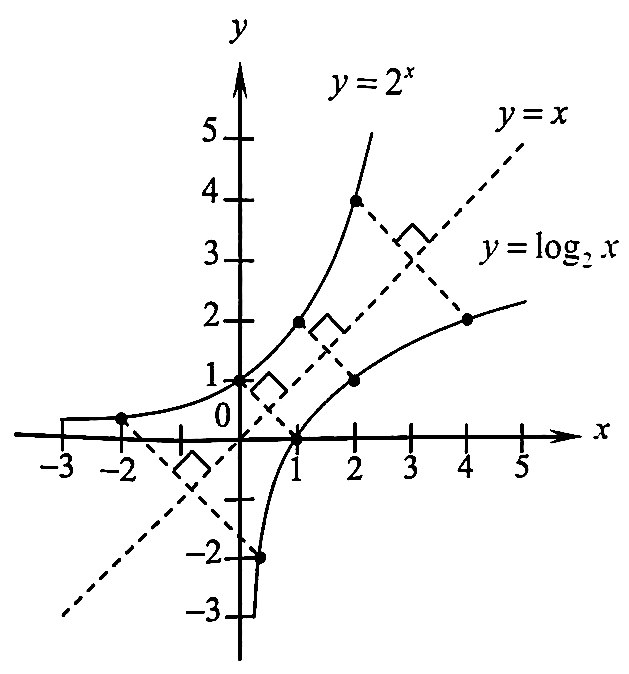
\includegraphics[scale=0.3]{./assets/log1.jpg}
    \hspace{1cm}
    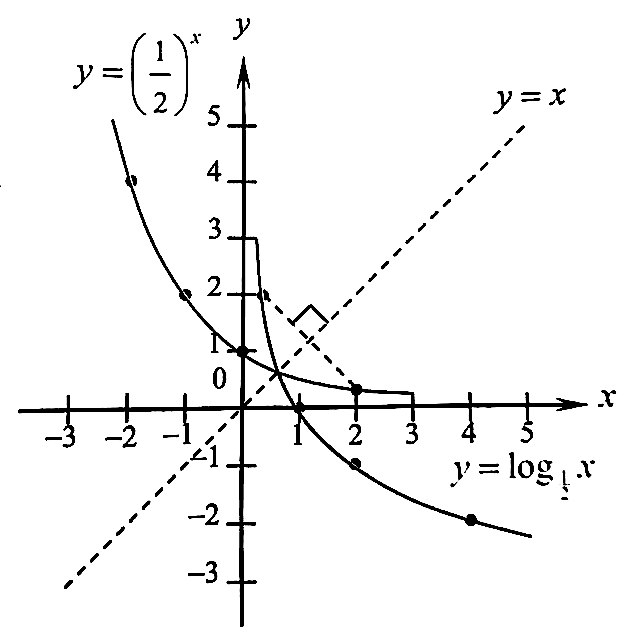
\includegraphics[scale=0.3]{./assets/log2.jpg}
\end{center}

From the diagram above, we can see that:
\begin{enumerate}[label=(\arabic*)]
    \item Since the domain of $y = \log_a x$ is $x > 0$, so the graph of the function $y
              = \log_2 x$ and $y = \log_\frac{1}{2} x$ are only at the right side of the
          $y$-axis.
    \item When $x = 1$, $y = 0$. Hence, the graph of logarithmic functions $y = a^x$
          always passes through the point $(1, 0)$.

    \item For the function $y = \log_2 x$, when $x > 1$, $y > 0$; when $0 < x < 1$, $y <
              0$. When the value of $x$ increases, the value of $y$ increases, that is, the
          function is an increasing function in the interval $(0, +\infty)$.

    \item For the function $y = \log_\frac{1}{2} x$, when $x > 1$, $y < 0$; when $0 < x <
              1$, $y > 0$. When the value of $x$ increases, the value of $y$ decreases, that
          is, the function is a decreasing function in the interval $(0, +\infty)$.
\end{enumerate}

\newpage
When we are discussing about the graph and properties of a logarithmic function
$y = \log_a x$, the following two cases are considered:

\begin{center}
    \begin{NiceTabular}{*{3}{c}}[corners,hvlines]
        & $a > 1$ & $0 < a < 1$ \\
        \Block{}{Graph} & 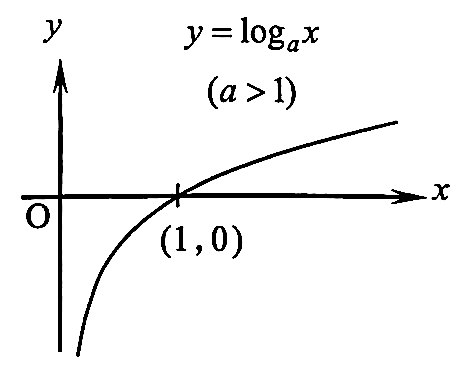
\includegraphics[scale=0.3]{assets/log3.jpg} & 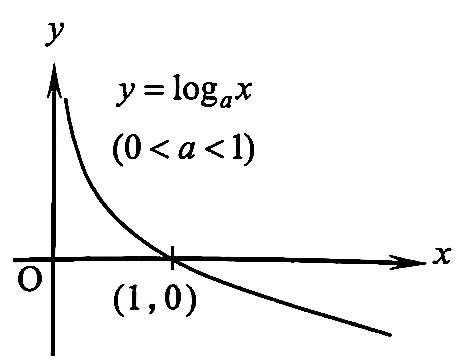
\includegraphics[scale=0.3]{assets/log4.jpg} \\
        \Block{4-1}{Properties} & \Block{1-2}{x > 0} \\
        & \Block{1-2}{When $x = 1$, $y = 0$} \\
        & \Block{}{When $x > 1$, $y > 0$;\\When $0 < y < 1$, $y < 0$} & \Block{}{When $x > 1$, $y < 0$;\\When $0 < x < 1$, $y > 0$} \\
        & \Block{}{It is an increasing function in \\the interval $(0, +\infty)$} & \Block{}{It is a decreasing function \\in the interval $(0, +\infty)$} \\
    \end{NiceTabular}
\end{center}
\newpage

\subsection*{Practice 4}

\begin{enumerate}
    \item Without using the calculator, Compare the value of the following expressions:
          \begin{enumerate}
              \begin{multicols}{2}
                  \item $\log 6$ and $\log 9$
                  \sol{}
                  \begin{flalign*}
                      \because\    & 10 > 1,\ y = \log{x} \text{ is an increasing}  & \\
                                   & \text{function in the interval } (0, +\infty),   \\
                      \because\    & 6 < 9,                                           \\
                      \therefore\  & \log{6} < \log{9}
                  \end{flalign*}

                  \item $\log_{0.5} 4.2$ and $\log_{0.5} 3.9$
                  \sol{}
                  \begin{flalign*}
                      \because\    & 0 < 0.5 < 1,\ y = \log{x} \text{ is a decreasing} & \\
                                   & \text{function in the interval } (-\infty, 0),      \\
                      \because\    & 4.2 > 3.9,                                          \\
                      \therefore\  & \log_{0.5} 4.2 < \log_{0.5} 3.9
                  \end{flalign*}
              \end{multicols}

              \item $\log_2 1.8$ abd $\log_4 5.8$.
                    \sol{}
                    \begin{flalign*}
                        \because\    & \log_2 1.8 < 1,\ \log_4 5.8 > 1, & \\
                        \therefore\  & \log_2 1.8 < \log_4 5.8
                    \end{flalign*}
          \end{enumerate}
    \item Find the domain of the following functions:
          \begin{enumerate}
              \begin{multicols}{2}
                  \item $y = \log_a(x+2)$
                  \sol{}
                  \begin{flalign*}
                      x + 2                     > 0 & \implies x > -2 \\
                      \therefore\ \text{Domain}     & = (-2, +\infty)
                  \end{flalign*}

                  \item $y = \log_2(x^2 - 9)$
                  \sol{}
                  \begin{flalign*}
                      x^2 - 9                   > 0 & \implies x < -3 \text{ or } x > 3 \\
                      \therefore\ \text{Domain}     & = (-\infty, -3) \cup (3, +\infty)
                  \end{flalign*}
              \end{multicols}

              \begin{multicols}{2}
                  \item $y = \log_7\dfrac{2}{3-2x}$
                  \sol{}
                  \begin{flalign*}
                      3 - 2x                    > 0 & \implies x < \dfrac{3}{2}            \\
                      \therefore\ \text{Domain}     & = \left(-\infty, \dfrac{3}{2}\right)
                  \end{flalign*}

                  \item $y - \sqrt{\log_5(2-x)}$
                  \sol{}
                  \begin{flalign*}
                      2 - x                     > 0 & \implies x < 2 \\
                      \therefore\ \text{Domain}     & = (-\infty, 2)
                  \end{flalign*}
              \end{multicols}
          \end{enumerate}
\end{enumerate}

\newpage
\subsection*{Exercise 23.2}

\begin{enumerate}
    \item Find the value of $x$ for the following expression:
          \begin{enumerate}
              \begin{multicols}{2}
                  \item $\log_2 x = 4$
                  \sol{}
                  \begin{flalign*}
                      \log_2 x & = 4   & \\
                      x        & = 2^4   \\
                               & = 16
                  \end{flalign*}
                  \vfill\null
                  \columnbreak
                  \item $\log_{125} x = \dfrac{1}{3}$
                  \sol{}
                  \begin{flalign*}
                      \log_{125} x & = \dfrac{1}{3}      & \\
                      x            & = 125^{\frac{1}{3}}   \\
                                   & = 5
                  \end{flalign*}
              \end{multicols}

              \begin{multicols}{2}
                  \item $\log_{16}(2\sqrt{2}) = x$
                  \sol{}
                  \begin{flalign*}
                      \log_{16}(2\sqrt{2}) & = x                                     & \\
                      x                    & = \log_{16}(2\sqrt{2})                    \\
                                           & = \log_{16}2 + \log_{16}\sqrt{2}          \\
                                           & = \log_{16}2 + \dfrac{1}{2}\log_{16}2     \\
                                           & = \dfrac{3}{2}\log_{16}2                  \\
                                           & = \dfrac{3}{2}\log_{16}16^{\frac{1}{4}}   \\
                                           & = \dfrac{3}{2}\cdot\dfrac{1}{4}           \\
                                           & = \dfrac{3}{8}
                  \end{flalign*}
                  \vfill\null
                  \columnbreak
                  \item $\log_\frac{1}{3}81 = x$
                  \sol{}
                  \begin{flalign*}
                      \log_\frac{1}{3}81 & = x                                                \\
                      x                  & = \log_\frac{1}{3}81                             & \\
                                         & = \log_\frac{1}{3}\left(\dfrac{1}{3}\right)^{-4}   \\
                                         & = -4
                  \end{flalign*}
              \end{multicols}

              \begin{multicols}{2}
                  \item $\log_x 81 = 4$
                  \sol{}
                  \begin{flalign*}
                      \log_x 81 & = 4            & \\
                      x^4       & = 81             \\
                      x         & = \sqrt[4]{81}   \\
                                & = 3
                  \end{flalign*}
                  \vfill\null
                  \columnbreak
                  \item $\log_x 49 = -2$
                  \sol{}
                  \begin{flalign*}
                      \log_x 49 & = -2                   & \\
                      x^{-2}    & = 49                     \\
                      x         & = \dfrac{1}{\sqrt{49}}   \\
                                & = \dfrac{1}{7}
                  \end{flalign*}
              \end{multicols}
          \end{enumerate}

          \newpage
    \item Sketch the graph of the following functions on the same set of axes:
          \begin{enumerate}
              \item $y = \log_5 x$
              \item $y = \log_\frac{1}{5} x$
          \end{enumerate}
          \sol{}
          \begin{center}
              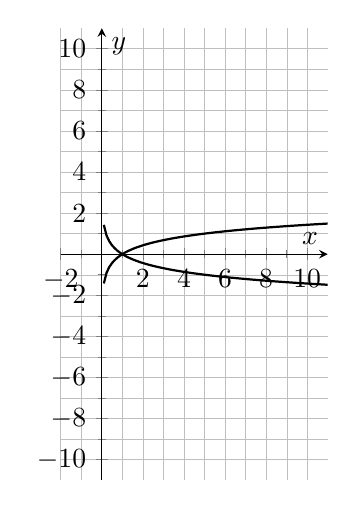
\begin{tikzpicture}
                  \begin{axis}[
                          unit vector ratio*=1 1 1,
                          axis lines = middle,
                          xlabel = $x$,
                          ylabel = $y$,
                          ymin = -11,
                          ymax = 11,
                          xmin = -2,
                          xmax = 11,
                          xtick = {-2, 0,...,10},
                          ytick = {-10,-8,...,10},
                          minor tick num = 1,
                          grid = both,
                          grid style = {line width=.1pt, draw=gray!50},
                          major grid style = {line width=.2pt,draw=gray!50},
                          width = 0.7\textwidth,
                      ]
                      \addplot [
                          domain=-2:11,
                          samples=100,
                          thick,
                      ]
                      {log10(x)/log10(5)};
                      \addplot [
                          domain=-2:11,
                          samples=100,
                          thick,
                      ]
                      {log10(x)/log10(1/5)};
                  \end{axis}
              \end{tikzpicture}
          \end{center}

    \item Without using the calculator, compare the value of the following expressions:
          \begin{enumerate}
              \begin{multicols}{2}
                  \item $\log_3 5$ and $\log_3 6$
                  \begin{flalign*}
                      \because\    & 3 > 1,\ y = \log{x} \text{ is an increasing}   & \\
                                   & \text{function in the interval } (0, +\infty),   \\
                      \because\    & 5 < 6,                                           \\
                      \therefore\  & \log{5} < \log{6}
                  \end{flalign*}

                  \item $\log_{1.5} 1.4$ and $\log_{1.5} 1.6$
                  \sol{}
                  \begin{flalign*}
                      \because\    & 1.5 > 1,\ y = \log{x} \text{ is an increasing} & \\
                                   & \text{function in the interval } (0, +\infty),   \\
                      \because\    & 1.4 < 1.6,                                       \\
                      \therefore\  & \log_{1.5}{1.4} < \log_{1.5}{1.6}
                  \end{flalign*}
              \end{multicols}

              \begin{multicols}{2}
                  \item $\log_{\sqrt{3}} 4.8$ and $\log_{\sqrt{3}} 5.8$
                  \sol{}
                  \begin{flalign*}
                      \because\    & \sqrt{3} > 1,\ y = \log{x} \text{ is an increasing} & \\
                                   & \text{function in the interval } (0, +\infty),        \\
                      \because\    & 4.8 < 5.8,                                            \\
                      \therefore\  & \log_{\sqrt{3}}{4.8} < \log_{\sqrt{3}}{5.8}
                  \end{flalign*}

                  \item $\log_{2.3} \pi$ and $\log_{2.3} (\pi - 3)$
                  \sol{}
                  \begin{flalign*}
                      \because\    & 2.3 > 1,\ y = \log{x} \text{ is an increasing} & \\
                                   & \text{function in the interval } (0, +\infty),   \\
                      \because\    & \pi > \pi - 3,                                   \\
                      \therefore\  & \log_{2.3}{\pi} > \log_{2.3}{(\pi - 3)}
                  \end{flalign*}
              \end{multicols}

              \begin{multicols}{2}
                  \item $\log_{0.4}\sqrt{2}$ and $\log_{0.4}\sqrt{3}$
                  \sol{}
                  \begin{flalign*}
                      \because\    & 0.4 < 1,\ y = \log{x} \text{ is a decreasing}  & \\
                                   & \text{function in the interval } (-\infty, 0),   \\
                      \because\    & \sqrt{2} < \sqrt{3},                             \\
                      \therefore\  & \log_{0.4}{\sqrt{2}} > \log_{0.4}{\sqrt{3}}
                  \end{flalign*}
                  \item $\log_\frac{1}{2} 3$ and $\log_\frac{1}{3} \dfrac{1}{4}$
                  \sol{}
                  \begin{flalign*}
                      \because\    & \frac{1}{2} < 1,\ y = \log{x} \text{ is a decreasing}       & \\
                                   & \text{function in the interval } (-\infty, 0),                \\
                      \because\    & \log_\frac{1}{2} 3 > 1,\ \log_\frac{1}{3} \dfrac{1}{4} < 1,   \\
                      \therefore\  & \log_\frac{1}{2} 3 < \log_\frac{1}{3} \dfrac{1}{4}
                  \end{flalign*}
              \end{multicols}
          \end{enumerate}

    \item Find the domain of the following functions:
          \begin{enumerate}
              \begin{multicols}{2}
                  \item $y = \log_2 (3-2x)$
                  \sol{}
                  \begin{flalign*}
                      3-2x                     > 0 & \implies x < \frac{3}{2}            & \\
                      \therefore\ \text{Domain}    & = \left(-\infty, \frac{3}{2}\right)
                  \end{flalign*}
                  \vfill\null
                  \columnbreak
                  \item $y = \log(x^2 + 1)$
                  \sol{}
                  \begin{flalign*}
                      x^2 + 1 > 0               & \text{ for all } x \in \mathbb{R}, & \\
                      \therefore\ \text{Domain} & = \mathbb{R}
                  \end{flalign*}
              \end{multicols}

              \begin{multicols}{2}
                  \item $y = \log_5(9-16x^2)$
                  \sol{}
                  \begin{flalign*}
                      9-16x^2 > 0               & \implies -\frac{3}{4} < x < \frac{3}{4}  & \\
                      \therefore\ \text{Domain} & = \left(-\frac{3}{4}, \frac{3}{4}\right)
                  \end{flalign*}
                  \vfill\null
                  \columnbreak
                  \item $y = \log_9 \dfrac{1}{x-2}$
                  \sol{}
                  \begin{flalign*}
                      x - 2 > 0                 & \implies x > 2 & \\
                      \dfrac{1}{x-2} > 0        & \implies x > 2   \\
                      \therefore\ \text{Domain} & = (2, +\infty)
                  \end{flalign*}
              \end{multicols}

              \begin{multicols}{2}
                  \item $y = \log_8 \sqrt{2x^2 - x - 3}$
                  \sol{}
                  \begin{flalign*}
                      2x^2 - x - 3 > 0          & \implies x < -1 \text{ or } x > \frac{3}{2}                       & \\
                      \therefore\ \text{Domain} & = \left(-\infty, -1\right) \cup \left(\frac{3}{2}, +\infty\right)
                  \end{flalign*}
                  \vfill\null
                  \columnbreak
                  \item $y = \dfrac{1}{\log_3 (7x-5)}$
                  \sol{}
                  \begin{flalign*}
                      \left\{\arraycolsep=1.4pt\def\arraystretch{1.5}
                      \begin{array}{l}
                          7x - 5 > 0        \\
                          \log_3 (7x-5) > 0 \\
                      \end{array}\right. & \implies x > \frac{5}{7},\ x \neq \frac{6}{7}                            &                   \\
                      \therefore\ \text{Domain}              & = \left(\frac{5}{7}, +\infty\right) \setminus \left\{\frac{6}{7}\right\}
                  \end{flalign*}
              \end{multicols}
          \end{enumerate}
\end{enumerate}

\section{Arithmetic Properties of Logarithms and Base Changing Formula}

\subsection*{Identties and Arithmetic Properties of Logarithms}

Logarithms have the following identities:
\begin{mdframed}[style=MyFrame]
    \setlength{\abovedisplayshortskip}{0pt}
    \setlength{\belowdisplayshortskip}{0pt}
    \setlength{\abovedisplayskip}{0pt}
    \setlength{\belowdisplayskip}{0pt}
    \makeatletter
    \setbool{@fleqn}{false}
    \makeatother
    \begin{flalign*}
        \log_a 1 & = 0 \\
        \log_a a & = 1
    \end{flalign*}
    \makeatletter
    \setbool{@fleqn}{true}
    \makeatother
\end{mdframed}

\noindent Logarithms have the following arithmetic properties:
\begin{mdframed}[style=MyFrame]
    \setlength{\abovedisplayshortskip}{0pt}
    \setlength{\belowdisplayshortskip}{0pt}
    \setlength{\abovedisplayskip}{0pt}
    \setlength{\belowdisplayskip}{0pt}
    \makeatletter
    \setbool{@fleqn}{false}
    \makeatother
    \begin{flalign*}
         & \log_a(xy) = \log_a x + \log_a y \quad (x > 0, y > 0)          \\
         & \log_a \dfrac{x}{y} = \log_a x - \log_a y \quad (x > 0, y > 0) \\
         & \log_a x^n = n \log_a x \quad (x > 0)                          \\
         & a^{\log_a x} = x
    \end{flalign*}
    \makeatletter
    \setbool{@fleqn}{true}
    \makeatother
\end{mdframed}

\subsection*{Base Changing Formula}

The base of a logarithm can be changed from one to another. Let $\log_a x = n$,
then $a^n = x$. Change both sides of the equation to logarithm with base $b$,
we have
\begin{flalign*}
    \log_b a^n                                & = \log_b x                   \\
    n \log_b a                                & = \log_b x                   \\
    \because\ a \neq 1,\ \therefore\ \log_b a & \neq 0                       \\
    n                                         & = \dfrac{\log_b x}{\log_b a} \\
    \therefore\ \log_a x                      & = \dfrac{\log_b x}{\log_b a}
\end{flalign*}
The expression above is called the \textit{base changing formula}.

\noindent When $x = b$, we have $\log_a b = \dfrac{1}{\log_b a}$.

\noindent In this book, the value of logarithms are rounded to 4 decimal places.

\subsection*{Practice 5}

\subsection*{Exercise 23.2}

\setlength{\columnseprule}{1pt}
\setlength{\columnsep}{24pt}
\begin{multicols}{2}
    Without using the calculator, compare the value of the following expressions
    (Question 1 to 4):

    \begin{enumerate}
        \item $5^{2\log_5 4}$
        \item $4^{3\log_2 \sqrt{2}}$
        \item $2\log 5 - \log \dfrac{1}{3} + \dfrac{1}{2} \log\dfrac{16}{9}$
        \item $\dfrac{\log_4 27}{\log_2 3}$
        \item Given that $\log_2 4 = a$ and $\log_2 5 = b$. Express the following expressions
              in terms of $a$ and $b$:
              \begin{enumerate}
                  \item $\log_2 90$
                  \item $\log_3 270$
                  \item $\log_9 1.8$
              \end{enumerate}

        \item Given that $\log_{16}y = \dfrac{1}{2} + \log_4 x$. Express $x$ in terms of $y$.
    \end{enumerate}
\end{multicols}

\subsection*{Exercise 23.3}

\subsection*{Exercise 23.2}

\setlength{\columnseprule}{1pt}
\setlength{\columnsep}{24pt}
\begin{multicols}{2}
    Simplify the following expressions (Question 1 to 6):
    \begin{enumerate}
        \item $\log_2 4^x$
        \item $\log_2 {a^{\log_a 2}}$
        \item $3^{\log_3 x - \log_3 y}$
        \item $\log_3 {(9^x \times 27^y)}$
        \item $2^{-\log_8 x}$
        \item $3\log_4 2^x$
    \end{enumerate}
    Without using the calculator, evaluate the following expressions (Question 7 to 22):
    \begin{enumerate}
        \setcounter{enumi}{6}
        \item $\log_7{\sqrt[3]{49}}$
        \item $49^{\log_7 3}$
        \item $2^{2\log_2 7}+\left({\dfrac{1}{2}}\right)^{-\log_2 7}$
        \item $\log_{3}5-\log_{3} 15$
        \item $\dfrac{\log{\sqrt{3}}}{\log{\dfrac{1}{9}}}$
        \item $\log_{5}{\dfrac{1}{5}}+\log_{5}{{\sqrt[3]{5}}-\log_{5}25}$
        \item $\log_{3}{\sqrt[3]{27{\sqrt[4]{81}}}}$
        \item $\log\left(0.1\right)^{4}-\log{\sqrt[3]{0.001}}$
        \item $\dfrac{\log4+\log3}{1+\log0.4+{\dfrac{1}{2}}\log9}$
        \item $\log_{36}6-\log_{6}36-\log_{6}{\dfrac{1}{6}}$
        \item $\log_{2}{\dfrac{1}{25}}\log_{3}{\dfrac{1}{8}}\cdot\log_{5}{\dfrac{1}{9}}$
        \item $\log_{4}5\cdot\log_{5}6\cdot\log_{6}7\cdot\log_{7}8$
        \item $\log_{4}8-\log_{\frac{1}{9}}3-\log_{\sqrt{2}}4$
        \item $\left(\log_{2}3+\log_{2}{\sqrt{3}}\right)\log_{\sqrt{3}}2$
        \item $\dfrac{\log_{5}\sqrt{2}\cdot\log_{7}9}{\log_{7}\sqrt[3]{4}\cdot\log_{5}{\dfrac{1}{3}}}$
        \item ${\dfrac{1}{2}}\log{\dfrac{81}{17}}+2\log{\dfrac{5}{3}}-\log{\dfrac{17}{4}}+{\dfrac{3}{2}}\log17$
        \item Given that $\log_2 3 = a$ and $\log_2 5 = b$. Express $a$ and $b$ in terms of
              $\log_4 15$.
        \item Given that $\log_3 5 = m$ and $\log_5 6 = n$. Express $m$ and $n$ in terms of
              $\log_25 54$.
        \item Given that $\log_2 3 = a$ and $\log_3 7 = b$. Express $a$ and $b$ in terms of
              $\log_42 14$.
        \item Given that $\log_3 6 = x$. Epress $x$ in terms of $\log_9 12$.
        \item Given that $\log_3 y - \log_9 \sqrt[3]{x} = 1 + \log_27 x$. Exress $x$ in terms
              of $y$.
        \item Given that $\log_25(2x - 1) = \log_5(x-3) + \log_25 5$, prove that $5x^2 - 32x
                  + 46 = 0$.
        \item If $a > 0$, $b > 0$, and $a^2 + b^2 = 7ab$, prove that $2\log_3(a+b) = 2 +
                  \log_3 a + \log_3 b$.
        \item If $x > 0$, $y > 0$, and $x^2 + 9y^2 = 10xy$, prove that $2\log(x+3y) - 4\log2
                  = \log x + \log y$.
    \end{enumerate}
\end{multicols}

\section{Exponential Equations}

All the equations with terms that contain the variable in the exponent are
called exponential equations. For example, $9^x = 3^{x-1}$, $3^x = 5$, and
$2^{x-1} + 2^x - 2 = 0$ are all exponential equations.

\subsection*{Practice 6}

\setlength{\columnseprule}{1pt}
\setlength{\columnsep}{24pt}
\begin{multicols}{2}
    Solve the following exponential equations:
    \begin{enumerate}
        \item $3^{2x} = -\dfrac{1}{9}$
        \item $2^{x^2 + 4x} = \dfrac{1}{8}$
        \item $6^x = 5^{x-1}$
        \item $4^{x-1} + 2^{x-1} = 20$
    \end{enumerate}
\end{multicols}

\subsection*{Exercise 23.4}

\setlength{\columnseprule}{1pt}
\setlength{\columnsep}{24pt}
\begin{multicols}{2}
    Solve the following exponential equations:

    \begin{enumerate}
        \item $8^{x-3}=\dfrac{1}{256}$
        \item $3^{2x+1}=243$
        \item $10^{x^{2}-4}=1$
        \item $3^{x^{2}+3}=27^{x+7}$
        \item $4^{x^{2}}=2^{5x+7}$
        \item $5^{2x^{2}+x}=25^{1+x-2x^{2}}$
        \item $\left({\dfrac{9}{16}}\right)^{x}=\left({\dfrac{4}{3}}\right)^{x-6}$
        \item $5^{2^x+1}=5^{4^x+1}$
        \item $2^{2x+3}\cdot4^{x+6}=\left(8^{x}\right)^{x}$
        \item ${\dfrac{5^{x^{2}}}{5}}=7^{(x+1)(x-1)}$
        \item $3^{x+1}=4^{x-1}$
        \item $7^{5-3x}=5^{x+2}$
        \item $13^{2x+5}=14^{x+7}$
        \item $2^{x^{2}-1}=3^{x+1}$
        \item $\left({\dfrac{1}{3}}\right)^{x}-\left({\dfrac{1}{3}}\right)^{-x}={\dfrac{80}{9}}$
        \item $3^{x+1}+9^{x}-18=0$
        \item $25^{x}-23\cdot5^{x}-50=0$
        \item $3^{x-1}+3^{3-x}-10=0$
        \item $3^{2x}-3^{x+1}+2=0$
        \item $2^{x+2}+3\left(2^{1-x}\right)-14=0$
        \item $2^{2x-1}-3\cdot2^{x-1}+1=0$
        \item $3^{x}-5^{x+2}=3^{x+1}-5^{x+3}$
    \end{enumerate}
\end{multicols}

\section{Logarithmic Equations}

All the equations with logarithmic terms which contains variable in the base or
in the argument are called logarithmic equations. For example, $\log(x-1) = 3$,
$\log_x 9 = 2$, and $2\log_3 x + \log_9 x = 1$ are all logarithmic equations.
The results acquired when solving logarithmic equations need to be checked.

\subsection*{Practice 7}

\setlength{\columnseprule}{1pt}
\setlength{\columnsep}{24pt}
\begin{multicols}{2}

    Solve the following logarithmic equations:
    \begin{enumerate}
        \item $\log_3 x=5$
        \item $\log_{5}(x-2)=0$
        \item $\log(x^{2}+2x-3)-\log(x+3)=0$
        \item $\log_{3}(3x+1)+1=\log_{3}(2x-1)+\log_{3}5$
        \item $\log_{x}3+\log_{x}81=5$
        \item $3\log_{2}^{2}x+5\log_{2}x-2=0$
        \item $\log_{2}x-\log_{x}8=2$
        \item $x^{\log x}=100x$
    \end{enumerate}

\end{multicols}

\subsection*{Exercise 23.5}

\setlength{\columnseprule}{1pt}
\setlength{\columnsep}{24pt}
\begin{multicols}{2}
    Solve the following logarithmic equations:
    \begin{enumerate}
        \item $\log_{\sqrt{3}}x=-2$
        \item $\log_{2}x^{4}=4$
        \item $\log{\frac{x-2}{x+2}}=\log{\frac{1}{x-1}}$
        \item $2\log x+\log7=\log14$
        \item $\log x+\log\left(x-3\right)=1$
        \item $\log\left(x+6\right)-\log\left(x-3\right)=1$
        \item $\log_{6}x+\log_{6}(x^{2}-7)=1$
        \item $\log_{1,2}(15x^{2}-2x-12)=0$
        \item $\log_{8}(x^{2}-3x-2)={\frac{1}{3}}$
        \item $\log_{2}(x^{2}-x-2)-\log_{2}(x+1)=0$
        \item $\log_{3}(2x-3)+\log_{3}(3x+2)=\log_{3}(2x-1)$
        \item $\frac{1}{2}(\log x-\log5)=\log2-\frac{1}{2}\log(9-x)$
        \item $\log\left(x+6\right)-{\frac{1}{2}}\log\left(2x-3\right)=2-\log25$
        \item $\log_{2}x=\log_{8}x+1$
        \item $3^{\log x}=2^{\log3}$
        \item $4x^{\log_{2}x}=x^{3}$
        \item $2\bigl(\log_{3}x\bigr)^{2}+\log_{3}x-1=0$
        \item $\log_{4}^{2}x-5\log_{4}x+6=0$
        \item $6\log^{2}x+\log x^{3}-3=0$
        \item $(\log x)^{2}=2\log x$
        \item $\log_{x}25-\log_{25}x=0$
        \item $2\log_{4}x-3\log_{x}4+5=0$
        \item $2\log_{x}10-\log x+1=0$
        \item $\log_{5}\left[\log_{2}\left(\log_{x}5\right)\right]=0$
    \end{enumerate}
\end{multicols}

\section{Compound Interest and Annuity}

Simple interest and compound interest are two different methods of calculating
interest. Simple interest is calculated on the principal amount of a loan only.
Compound interest is calculated on the principal amount and also on the
accumulated interest of previous periods, and can thus be regarded as “interest
on interest.”

For example, a fund amounted to RM$p$ is deposited into a bank account with a
yearly interest rate of $r\%$.
\begin{flalign*}
    \text{Principal amount} & = \text{RM} p
\end{flalign*}
When $t = 1$,
\begin{flalign*}
    \text{Interest earned}    & = p \times r\% = \frac{pr}{100}                        \\
    \text{Accumulated amount} & = p + \frac{pr}{100} = p\left(1 + \frac{r}{100}\right)
\end{flalign*}
When $t = 2$,
\begin{flalign*}
    \text{Interest earned}    & = \left(p + \frac{pr}{100}\right) \times r\% = \frac{pr}{100}\left(1 + \frac{r}{100}\right) \\
    \text{Accumulated amount} & = p\left(1 + \frac{r}{100}\right) + \frac{pr}{100}\left(1 + \frac{r}{100}\right)            \\
                              & = p\left(1 + \frac{r}{100}\right)\left(1 + \frac{r}{100}\right)                             \\
                              & = p\left(1 + \frac{r}{100}\right)^{2}
\end{flalign*}
When $t = 3$,
\begin{flalign*}
    \text{Interest earned}    & = \left(p\left(1 + \frac{r}{100}\right)^{2}\right) \times r\% = \frac{pr}{100}\left(1 + \frac{r}{100}\right)^{2} \\
    \text{Accumulated amount} & = p\left(1 + \frac{r}{100}\right)^{2} + \frac{pr}{100}\left(1 + \frac{r}{100}\right)^{2}                         \\
                              & = p\left(1 + \frac{r}{100}\right)^{2}\left(1 + \frac{r}{100}\right)                                              \\
                              & = p\left(1 + \frac{r}{100}\right)^{3}
\end{flalign*}

In general, the accumulated amount after $t$ years is given by
\begin{mdframed}[style=MyFrame]
    \setlength{\abovedisplayshortskip}{0pt}
    \setlength{\belowdisplayshortskip}{0pt}
    \setlength{\abovedisplayskip}{0pt}
    \setlength{\belowdisplayskip}{0pt}
    \makeatletter
    \setbool{@fleqn}{false}
    \makeatother
    \begin{flalign*}
        A & = p\left(1 + \frac{r}{100}\right)^{t}
    \end{flalign*}
    \makeatletter
    \setbool{@fleqn}{true}
    \makeatother
\end{mdframed}
where $p$ is called the \textit{present value} of $A$.

If the interest is compounded $m$ times per year, then the accumulated amount
is given by
\begin{mdframed}[style=MyFrame]
    \setlength{\abovedisplayshortskip}{0pt}
    \setlength{\belowdisplayshortskip}{0pt}
    \setlength{\abovedisplayskip}{0pt}
    \setlength{\belowdisplayskip}{0pt}
    \makeatletter
    \setbool{@fleqn}{false}
    \makeatother
    \begin{flalign*}
        A & = p\left(1 + \frac{r}{100m}\right)^{mt}
    \end{flalign*}
    \makeatletter
    \setbool{@fleqn}{true}
    \makeatother
\end{mdframed}

\subsection*{Annuity and Present Value of Annuity}

An annuity is a series of equal payments made at equal intervals of time
according to some kind of contract, standing order or the amount received. For
example, all sorts of instalment, insurance premiums, house rent, car loan,
etc. are annuities. In this book, we will only consider annuities with equal
payments made or received at equal intervals of time.

Note that the annuity is not limited to once a year.

We can compare which payment plan is better by comparing the present values of
the annuities. From the formula $A = p\left(1 + r\%\right)^{t}$, we can know
that the present value $p = \dfrac{A}{\left(1 + r\%\right)^{t}}$. If the yearly
interest rate is $r\%$, the annuity is RM$A$, the payment is made once per
year, then the present value of the amount paid after a year is $A(1 +
    r\%)^{-1}$, the present value of the amount paid after two years is $A(1 +
    r\%)^{-2}$, and so on. The present value of the amount paid after $n$ years is
$A(1 + r\%)^{-n}$. Hence, the sum of the present values of the amount paid
after $n$ years is
\begin{flalign*}
     & \dfrac{A}{1+r\%} + \dfrac{A}{(1+r\%)^2} + \cdots + \dfrac{A}{(1+r\%)^n}                 \\
     & = A\left[\dfrac{1}{1+r\%} + \dfrac{1}{(1+r\%)^2} + \cdots + \dfrac{1}{(1+r\%)^n}\right] \\
     & = A\left[\dfrac{1-\dfrac{1}{(1+r\%)^n}}{1-\dfrac{1}{1+r\%}}\right]                      \\
     & = \dfrac{A}{r\%}\left(1 - \dfrac{1}{(1+r\%)^n}\right)
\end{flalign*}

Annuity that is paid indefinitely is called \textit{perpetuity}, $n \to
    \infty$, $\dfrac{1}{(1+r\%)^n} \to 0$. From that, we can know that the present
value of perpetuity is $\dfrac{A}{r\%}$.

\subsection*{Practice 8}

\setlength{\columnseprule}{1pt}
\setlength{\columnsep}{24pt}
\begin{multicols}{2}
    \begin{enumerate}
        \item Given that the principal amount is RM75,000, interest rate is 4.5\%. Using
              composite interest method, find the accumulated amount after 10 years.
        \item A person has deposited RM40,000 into a bank account. The bank pays 8\% interest
              per annum compounded half yearly. Using the compound interest method, find the
              amount in the account after 3 years.
        \item Given that the interest rate is 6\%, the interest is compounded half yearly.
              Using the compound interest method, the accumulated amount after 5 years is
              RM4031.75, find the principal amount.
        \item Given that the interest rate is 4\%, the annuity is RM3,500, the payment is
              made once per year. The payment has since been made for 15 years continuously.
              Find the present value. Hence, find the present value of the perpetuity.
    \end{enumerate}
\end{multicols}

\subsection*{Exercise 23.6}

\setlength{\columnseprule}{1pt}
\setlength{\columnsep}{24pt}
\begin{multicols}{2}
    \begin{enumerate}
        \item Given that the principal amount is RM90,000, the interest rate is 5\%.
              Compounding the interest once per year, find the accumulated amount after 10
              years.
        \item A person has deposited a fund into a bank account. The bank pays 8\% interest
              per annum compounded yearly. The amount in the account after 3 years has
              increased by RM779.14. Find the amount of the fund deposited.

        \item RM80,000 was deposited into a financial institution. The interest rate is 8\%
              per annum compounded once per three months. Find the amount in the account
              after 5 years.
        \item Prove that the accumulated amount after being compounded with an interest of
              $5$ for 15 years will exceed twice the principal amount.
        \item Given that the principal amount is RM15,000, the interest rate is 6\% being
              compouned once per year. How long does it take for the accumulated amount to be
              more than RM30,000?
        \item Given that the principal amount is RM120,000, the interest rate is 5.5\% being
              compounded half yearly. How long does it take for the accumulated amount to be
              more than RM200,000?
        \item A person deposited RM2,500 into his bank account at the beginning of the yaar,
              the interest rate is 4.5\% compounded once per year. Find the amount in the
              account after 15 years.
        \item If the present value is RM15,443.46, the interest rate is 5\%, find the annuity
              if the payment is made for 10 years.
        \item Given that the annuity is RM5,000, the interest rate is 5\%, the payment is
              made once per year for 25 years. Find the present value. Hence, find the
              present value of the perpetuity.
        \item Given that the annuity is RM2,500, the interest rate is 4.5\%, the payment is
              made once per year. How many years does it take for the present value to exceed
              RM30,000?
        \item If a bank has introduced an annuity scheme, the investors can receive RM1,000
              per year for life after paying RM20,000. If the annuity plan is considered
              approximately to be a perpetuity, find the interest rate.
    \end{enumerate}
\end{multicols}

\section*{Revision Exercise 23}
\setlength{\columnseprule}{1pt}
\setlength{\columnsep}{24pt}
\begin{multicols}{2}
    \begin{enumerate}
        \item Without using a calculator, find the value of the following:
              \begin{enumerate}
                  \item $\left({\frac{1}{2}}\right)^{2}+\left({\frac{1}{2}}\right)^{6}+\left(-{\frac{1}{2}}\right)^{-2}$
                  \item $5^{\frac{1}{2}}+5^{-{\frac{1}{2}}}-\left(\dfrac{1}{5}\right)^{\frac{1}{2}}+\left(\dfrac{1}{5}\right)^{-{\frac{1}{2}}}$
                  \item $\left({\frac{1}{3}}\right)^{2}\times\left(-{\frac{1}{3}}\right)^{2}\times\left({\frac{1}{2}}\right)^{-2}$
                  \item ${\sqrt{2{\sqrt[3]{3}}}}\div{\sqrt[3]{\dfrac{\sqrt{8}}{3}}}$
              \end{enumerate}

        \item Simplify the following expressions:
              \begin{enumerate}
                  \item $\left({\dfrac{b}{2a^{2}}}\right)^{3}\div\left({\dfrac{2b^{2}}{3a}}\right)^{0}\times\left(-{\dfrac{b}{a}}\right)^{-3}$
                  \item $\dfrac{3^{n+2}-2\times3^{n}}{5(3^{n+1})}$
                  \item $\dfrac{\left(x^{-1}+y^{-1}\right)\left(x^{-1}-y^{-1}\right)}{x^{-2}y^{-2}}$
                  \item $\left({x^{\frac{1}{4}}}-y^{-{\frac{1}{4}}}\right)\left(x^{\frac{1}{2}}+y^{-{\frac{1}{2}}}\right)\left(x^{\frac{1}{4}}+y^{-{\frac{1}{4}}}\right)$
                  \item $\frac{\left({\sqrt[4]{p^{3}}}\right)^{\frac{1}{6}}{\sqrt[9]{p^{-3}}}}{\left(\sqrt{p^{-7}}\right)^{\frac{1}{6}}}$
                  \item $\dfrac{\left(a^{2}+a^{-2}+2\right)^{2}}{\left(a^{2}+1\right)^{4}}$
              \end{enumerate}

        \item Without using a calculator, compare the value of the following:
              \begin{enumerate}
                  \item $2.3^{-2}$ and $2.3^{-1}$
                  \item $0.15^{-{\frac{1}{2}}}$ and ${0.15}^{-{\frac{1}{3}}}$
                  \item $\left({\dfrac{1}{3}}\right)^{\frac{2}{5}}$ and $ 3^{-{\frac{5}{3}}}$
                  \item $\left({\dfrac{3}{5}}\right)^{2}$ and $\left({\dfrac{5}{3}}\right)^{3.1}$
              \end{enumerate}

        \item Without using a calculator, compare the value of the following:
              \begin{enumerate}
                  \item $\log_{3.2}3$ and $\log_{3.2}2$
                  \item $\log_{0.5}5.3$ and $\log_{0.5}3.5$
                  \item $\log_{3}2$ and $\log_{2}3$
                  \item $\log_{2}2.3$ and $\log_{4}4.8$
              \end{enumerate}

        \item Find the domain of the following functions:
              \begin{enumerate}
                  \item $y=\log_{0.5}\left(16-x^{2}\right)$
                  \item $y=\log_{2}\left(2x^{2}-5x-12\right)$
                  \item $y=\sqrt{3-3^{x}}$
                  \item $y=\log_{2}(x-3)^{2}$
                  \item $y=\log_{5}\left(x^{2}-2x\right)$
                  \item $y=\log_{3}{\dfrac{2}{3-x}}$
                  \item $y=\dfrac{1}{\log(x+1)-1}$
                  \item $y=\dfrac{\log_3\left(2-x\right)}{\log_3\left(2+x\right)}$
                  \item $y=\sqrt{\log_{3}(x-2)}$
                  \item $y={\dfrac{2}{\sqrt{1-\log x}}}$
              \end{enumerate}

        \item Simplify the following expressions:
              \begin{enumerate}
                  \item $\log_{3}27^{x}$
                  \item $\log_{x}b^{a\log_{b}x}$
                  \item $\log_{5}\left(25^{x}\cdot5^{y}\right)$
                  \item $3^{2\log_{3}x - \log_{3}y}$
                  \item $5^{-2\log_{25}x}$
              \end{enumerate}

        \item If $\log_2 5 = p$, express $\log_2 100$ in terms of $p$.
        \item If $\log_3 12 = a$, express the following in terms of $a$:
              \begin{enumerate}
                  \item $\log_3 24$
                  \item $\log_9 36$
              \end{enumerate}

        \item Without using a calculator, find the value of the following:
              \begin{enumerate}
                  \item $\log_{c}{\frac{1}{5}}+\log_{c}5$
                  \item $\log_{2}\left(2{\sqrt{2}}\right)-2\log_{2}{\sqrt{2}}$
                  \item $\log_8{\dfrac{2}{7}}-\log_{8}(-2)^{2}-\log_{8}{\dfrac{1}{7}}$
                  \item $\log{\dfrac{5}{32}}-2\log{\dfrac{5}{6}}+\log{\dfrac{40}{9}}$
                  \item ${\big(}\log_{2}3{\big)}{\big(}\log_{3}4{\big)}$
                  \item $\dfrac{\log_{16}5}{\log_{32}5}$
                  \item $\log_{3}5\cdot\log_{5}7\cdot\log_{7}27$
                  \item $\log_{2}{\dfrac{1}{9}}\cdot\log_{3}{\dfrac{1}{25}}\cdot\log_{5}\sqrt8$
                  \item $\dfrac{1}{3}\log_{2}8+\log_{3}27-\dfrac{1}{4}\log_{4}16$
                  \item $\log^{2}2+\log2\cdot\log5+\log5$
                  \item $2\log_{3}15+3\log_{3}12-\log_{3}25-6\log_{3}2$
                  \item ${\dfrac{\log{\sqrt{27}}+\log{\sqrt{8}}-\log{\sqrt{125}}}{\log6-\log5}}$
                  \item \resizebox{15.5em}{!}{$\log_{8}\left(\log_{2}{\sqrt{8+4{\sqrt{3}}}}+\log_{2}{\sqrt{8-4\sqrt{3}}}\right)$}
              \end{enumerate}

        \item If $\log_3 2 = a$, $\log_2 5 = b$, prove that $\log_5 3 = \dfrac{1}{a(b+1)}$.
        \item If $\log_2 3 = p$, $\log_3 7 = q$, prove that $\log_21 14 =
                  \dfrac{pq+1}{p(q+1)}$.
        \item Given that $2\log_5(x+y) = 1 + \log_5 x + \log_5 y$. Prove that $x^2 + y^2 =
                  3xy$.
        \item Given that $x = 5^k$ and $y = 5^n$. Express the following in terms of $k$ and
              $n$:
              \begin{enumerate}
                  \item $\log_{5}{\dfrac{xy^3}{125}}$
                  \item $\log_{25}\left(5{\sqrt{xy}}\right)$
              \end{enumerate}

        \item Given that $2 + \log_4 y = 2\log_16 x$. Express $x$ in terms of $y$.

        \item Solve the following exponential equations:
              \begin{enumerate}
                  \item $3^{3x-2}=243$
                  \item $4^{1-x}=\left({\dfrac{1}{8}}\right)^{2}$
                  \item $2^{x^{2}}=\left(2^{x}\right)^{2}$
                  \item $3^{5^x}=3$
                  \item $5^{8^x}=625$
                  \item $3^{x+1}=6^{x}$
                  \item $7^{x}-7^{x-1}=6$
                  \item $3^{x+1}=10\left(3^x\right)-3$
                  \item $2^{2x+1}=3\left(2^{x}\right)-1$
                  \item $5^{2x+1}=26\left(5^{x}\right)-5$
                  \item $2^{2x+3}-2^{x}=1-2^{x+3}$
                  \item $2^{2x+8}-32\left(2^{x}\right)+1=0$
              \end{enumerate}

        \item If $\log_2 x + \log_4 x = \dfrac{9}{2}$, find the value of $x$.
        \item Solve the follwoing logarithmic equations:
              \begin{enumerate}
                  \item $2\log x-3\log4=2$
                  \item $2\log x=\log32+\log2$
                  \item $\log x+\log\left(x+3\right)=\log\left(x+8\right)$
                  \item $\left(\log_{2}x\right)^{2}=\log_{2}x+6$
                  \item $\log_{3}x+6\log_{x}3=5$
                  \item $4^{\log x}=2^{\log x+1}$
                  \item $\log_{x+1}\left(x^{2}-5x-13\right)=2$
                  \item $\log_{r}{\sqrt{2x^{2}-5x+6}}=1$
                  \item $\log_{2}(x+1)+\log_{2}(x+3)=3+\log_{2}x$
                  \item $\log_{2}\left[\log_{3}\left(\log_{5}x\right)\right]=0$
                  \item $3\log_{s}x-2\log_{2}x+2=0$
                  \item $\log_{4}(x+4)+1=\log_{2}(x+1)$
                  \item $2\log_{2}x\cdot\log_{8}x=\log_{2}x+\log_{8}x$
              \end{enumerate}

        \item A person has deposited a fund into a bank account that pays 5.5\% interest
              compounded annually. If the balance in the account has increased by RM1,432.95
              after 4 years, how much was deposited initially?

        \item Given that there is a principal of RM75,000 at an interest rate of 3.5\% per
              annum compounded once per three months. Find the accumulated value of the
              principal after 8 years.

        \item Given that there is a principal of RM150,000 at an interest rate of 5.25\% per
              annum compounded once per annum. How many years does it take to accumulate at
              least RM300,000?

        \item If the present value is RM24,924.44, the interest rate is 5\% per annum
              compounded once per annum, find the annuity payment if the payment is made for
              20 years.

        \item Given that the annuity payment is RM8,000, the interest rate is 4.5\% per annum
              compounded once per annum, and the payment is made for 15 years. Find the
              present value. Hence, find the present value of the perpetuity.

        \item Given that the annuity amount is RM4,500, the interest rate is 4.5\% per annum
              compounded once per annum. How many years does it take for the present value to
              exceed RM50,000?

        \item The price of a branded laptop is RM2,500, the payment can be paid in full or by
              instalment. If the payment is made by instalment, the monthly payment is RM110
              for 2 years. If the interest rate is 4\% per annum compounded once per month,
              which payment method is more economical considering the present value of the
              payment?
    \end{enumerate}
\end{multicols}

\end{document}